\documentclass[10pt]{article}
\usepackage{ctex}
\usepackage{CJK}
\usepackage{graphicx}
\usepackage{booktabs}
\bibliographystyle{plain}
\setlength{\parindent}{2em}
\begin{document}
\title{Optical systems}
\author{Qilei Zhang}
\date{may 27 2018}
\maketitle
\par
Stochastic resonance was realized in an electronic circuit,a simple Schmitt trigger (Fauve and Heslot, 1983). Since then, stochastic resonance has been observed in a variety of more or less complicated electronic devices, mostly constructed with the purpose of building flexible and inexpensive simulation tools.\cite{Alpher02}
\par
\begin{figure}[htbp]
\small
\centering
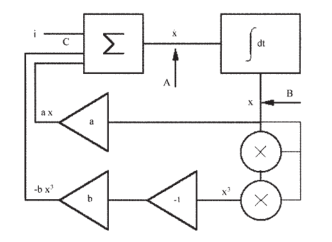
\includegraphics[width=20em]{023.png}
\caption{23 Bistable ring laser}
\label{fig:lable}
\end{figure}
\section{Analog electronic simulators}
As mentioned in Sec. II.C, electronic circuits have been widely employed in the study of nonlinear stochastic equations. The realization of an electronic simulation circuit requires the design of specific electronic devices which operate as the single components of the block scheme depicted in Fig. 23.
\section{Electron paramagnetic resonance}
An EPR system consists of a paramagnetic sample placed in a microwave cavity. A microwave generator irradiates the sample while a feedback electronic circuit locks the oscillator frequency to the resonant frequency Nc of the cavity.\cite{Alpher03}\\
$X(t)=-H(t)\sum_{n=1}^\infty g_n l_n exp(-l_n t)$\\
$\quad x'=x-x^3+u(t)+A_0 cos(st)$
\section{Superconducting quantum interference devices}
The basic components of a SQUID are a superconducting loop and a Josephson junction. For practical purposes, a SQUID can be envisioned as an electromagnetic device that converts a magnetic flux variation into a voltage variation and, as such, it has been successfully employed in monitoring small magnetic field fluctuations.\cite{Alpher04}\\
\begin{tabular}{cccccccc}
\toprule
         & 1 &  2  &   3  &  4  &  5  &  6  & 7 \\
\midrule
Alphabet & A &  B  &   C  &  D  &  E  &  F  & G\\
Roman    & I &  II &  III &  IV &  V  &  VI & VII\\
\bottomrule
\end{tabular}
\bibliography{zzz}
\end{document}

